% !TeX program = pdflatex
% !TeX root = FCGraphFindPath.tex

\documentclass[../FeynCalcManual.tex]{subfiles}
\begin{document}
\hypertarget{fcgraphfindpath}{
\section{FCGraphFindPath}\label{fcgraphfindpath}\index{FCGraphFindPath}}

\texttt{FCGraphFindPath[\allowbreak{}graph,\ \allowbreak{}weights]}
determines whether the given graph can be traversed by starting and
finishing at one of the external edges.

The respective external edges must differ and
\texttt{\{\allowbreak{}1\}} is returned for all graphs with less than
two such edges, since tadpoles have no cut by definition.

The only supported weights are 1 and -1, with -1 meaning that the given
edge cannot be passed.

Only directed graphs are supported but the direction of edges does not
matter when searching for the path. The path is understood to be free of
any cycles (loops).

\subsection{See also}

\hyperlink{toc}{Overview},
\hyperlink{fcgraphcuttableq}{FCGraphCuttableQ},
\hyperlink{fcloopintegraltograph}{FCLoopIntegralToGraph},
\hyperlink{samesideexternaledges}{SameSideExternalEdges}.

\subsection{Examples}

This integral has no imaginary part due to the massive \texttt{m1}-line
that cannot be cut

\begin{Shaded}
\begin{Highlighting}[]
\NormalTok{graph1 }\ExtensionTok{=} \OperatorTok{\{}\SpecialCharTok{{-}}\DecValTok{3} \OtherTok{{-}\textgreater{}} \DecValTok{2}\OperatorTok{,} \SpecialCharTok{{-}}\DecValTok{1} \OtherTok{{-}\textgreater{}} \DecValTok{1}\OperatorTok{,} \DecValTok{1} \OtherTok{{-}\textgreater{}} \DecValTok{3}\OperatorTok{,} \DecValTok{1} \OtherTok{{-}\textgreater{}} \DecValTok{4}\OperatorTok{,} \DecValTok{2} \OtherTok{{-}\textgreater{}} \DecValTok{3}\OperatorTok{,} \DecValTok{2} \OtherTok{{-}\textgreater{}} \DecValTok{4}\OperatorTok{,} \DecValTok{2} \OtherTok{{-}\textgreater{}} \DecValTok{4}\OperatorTok{,} \DecValTok{3} \OtherTok{{-}\textgreater{}} \DecValTok{4}\OperatorTok{\}}\NormalTok{;}
\end{Highlighting}
\end{Shaded}

\begin{Shaded}
\begin{Highlighting}[]
\FunctionTok{GraphPlot}\OperatorTok{[}\NormalTok{graph1}\OperatorTok{]}
\end{Highlighting}
\end{Shaded}

\FloatBarrier
\begin{figure}[!ht]
\centering
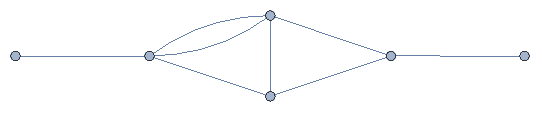
\includegraphics[width=0.6\linewidth]{img/1ak8ujeaxy5t3.pdf}
\end{figure}
\FloatBarrier

\begin{Shaded}
\begin{Highlighting}[]
\NormalTok{res1 }\ExtensionTok{=}\NormalTok{ FCGraphFindPath}\OperatorTok{[}\NormalTok{graph1}\OperatorTok{,} \OperatorTok{\{}\DecValTok{1}\OperatorTok{,} \DecValTok{1}\OperatorTok{,} \DecValTok{1}\OperatorTok{,} \DecValTok{1}\OperatorTok{,} \DecValTok{1}\OperatorTok{,} \SpecialCharTok{{-}}\DecValTok{1}\OperatorTok{,} \DecValTok{1}\OperatorTok{,} \SpecialCharTok{{-}}\DecValTok{1}\OperatorTok{\}]}
\end{Highlighting}
\end{Shaded}

\begin{dmath*}\breakingcomma
\left(
\begin{array}{cccc}
 \{-3\to 2,1\} & \{2\to 3,5\} & \{1\to 3,3\} & \{-1\to 1,2\} \\
 \{-3\to 2,1\} & \{2\to 4,7\} & \{1\to 4,4\} & \{-1\to 1,2\} \\
\end{array}
\right)
\end{dmath*}

\begin{Shaded}
\begin{Highlighting}[]
\FunctionTok{HighlightGraph}\OperatorTok{[}\NormalTok{graph1}\OperatorTok{,}\NormalTok{ res1}\OperatorTok{[[}\DecValTok{1}\OperatorTok{]],} \FunctionTok{GraphLayout} \OtherTok{{-}\textgreater{}} \StringTok{"SpringElectricalEmbedding"}\OperatorTok{]}
\end{Highlighting}
\end{Shaded}

\FloatBarrier
\begin{figure}[!ht]
\centering
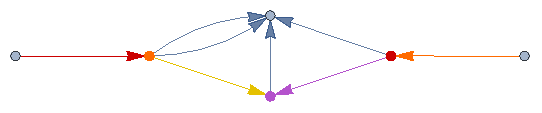
\includegraphics[width=0.6\linewidth]{img/1pgx7tpi7v61b.pdf}
\end{figure}
\FloatBarrier

\begin{Shaded}
\begin{Highlighting}[]
\FunctionTok{HighlightGraph}\OperatorTok{[}\NormalTok{graph1}\OperatorTok{,}\NormalTok{ res1}\OperatorTok{[[}\DecValTok{2}\OperatorTok{]],} \FunctionTok{GraphLayout} \OtherTok{{-}\textgreater{}} \StringTok{"SpringElectricalEmbedding"}\OperatorTok{]}
\end{Highlighting}
\end{Shaded}

\FloatBarrier
\begin{figure}[!ht]
\centering
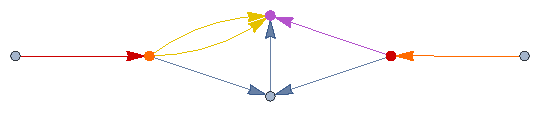
\includegraphics[width=0.6\linewidth]{img/0n46uoe6w24dg.pdf}
\end{figure}
\FloatBarrier

\begin{Shaded}
\begin{Highlighting}[]
\NormalTok{graph2 }\ExtensionTok{=} \OperatorTok{\{}\SpecialCharTok{{-}}\DecValTok{4} \OtherTok{{-}\textgreater{}} \DecValTok{4}\OperatorTok{,} \SpecialCharTok{{-}}\DecValTok{3} \OtherTok{{-}\textgreater{}} \DecValTok{1}\OperatorTok{,} \SpecialCharTok{{-}}\DecValTok{2} \OtherTok{{-}\textgreater{}} \DecValTok{2}\OperatorTok{,} \SpecialCharTok{{-}}\DecValTok{1} \OtherTok{{-}\textgreater{}} \DecValTok{3}\OperatorTok{,} \DecValTok{1} \OtherTok{{-}\textgreater{}} \DecValTok{4}\OperatorTok{,} \DecValTok{1} \OtherTok{{-}\textgreater{}} \DecValTok{6}\OperatorTok{,} \DecValTok{2} \OtherTok{{-}\textgreater{}} \DecValTok{3}\OperatorTok{,} 
    \DecValTok{2} \OtherTok{{-}\textgreater{}} \DecValTok{6}\OperatorTok{,} \DecValTok{3} \OtherTok{{-}\textgreater{}} \DecValTok{5}\OperatorTok{,} \DecValTok{4} \OtherTok{{-}\textgreater{}} \DecValTok{5}\OperatorTok{,} \DecValTok{5} \OtherTok{{-}\textgreater{}} \DecValTok{6}\OperatorTok{\}}\NormalTok{;}
\end{Highlighting}
\end{Shaded}

\begin{Shaded}
\begin{Highlighting}[]
\FunctionTok{GraphPlot}\OperatorTok{[}\NormalTok{graph2}\OperatorTok{,} \FunctionTok{VertexLabels} \OtherTok{{-}\textgreater{}} \StringTok{"Name"}\OperatorTok{]}
\end{Highlighting}
\end{Shaded}

\FloatBarrier
\begin{figure}[!ht]
\centering
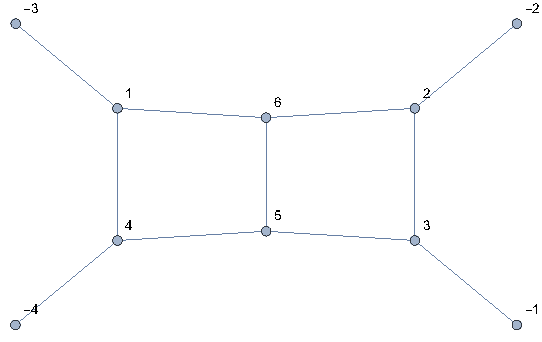
\includegraphics[width=0.6\linewidth]{img/0i0qkwnvhlnmi.pdf}
\end{figure}
\FloatBarrier

\begin{Shaded}
\begin{Highlighting}[]
\NormalTok{res2 }\ExtensionTok{=}\NormalTok{ FCGraphFindPath}\OperatorTok{[}\NormalTok{graph2}\OperatorTok{,} \OperatorTok{\{}\DecValTok{1}\OperatorTok{,} \DecValTok{1}\OperatorTok{,} \DecValTok{1}\OperatorTok{,} \DecValTok{1}\OperatorTok{,} \SpecialCharTok{{-}}\DecValTok{1}\OperatorTok{,} \SpecialCharTok{{-}}\DecValTok{1}\OperatorTok{,} \DecValTok{1}\OperatorTok{,} \SpecialCharTok{{-}}\DecValTok{1}\OperatorTok{,} \DecValTok{1}\OperatorTok{,} \SpecialCharTok{{-}}\DecValTok{1}\OperatorTok{,} \DecValTok{1}\OperatorTok{\}]}
\end{Highlighting}
\end{Shaded}

\begin{dmath*}\breakingcomma
\left(
\begin{array}{ccc}
 \{-2\to 2,3\} & \{2\to 3,7\} & \{-1\to 3,4\} \\
\end{array}
\right)
\end{dmath*}

\begin{Shaded}
\begin{Highlighting}[]
\FunctionTok{HighlightGraph}\OperatorTok{[}\NormalTok{graph2}\OperatorTok{,}\NormalTok{ res2}\OperatorTok{[[}\DecValTok{1}\OperatorTok{]],} \FunctionTok{GraphLayout} \OtherTok{{-}\textgreater{}} \StringTok{"SpringElectricalEmbedding"}\OperatorTok{]}
\end{Highlighting}
\end{Shaded}

\FloatBarrier
\begin{figure}[!ht]
\centering
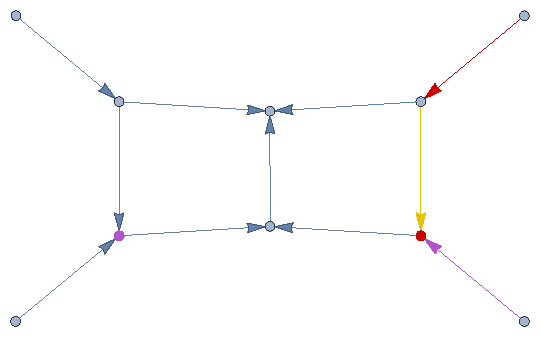
\includegraphics[width=0.6\linewidth]{img/0833y1scsk90z.pdf}
\end{figure}
\FloatBarrier

\begin{Shaded}
\begin{Highlighting}[]
\NormalTok{FCGraphFindPath}\OperatorTok{[}\NormalTok{graph2}\OperatorTok{,} \OperatorTok{\{}\DecValTok{1}\OperatorTok{,} \DecValTok{1}\OperatorTok{,} \DecValTok{1}\OperatorTok{,} \DecValTok{1}\OperatorTok{,} \SpecialCharTok{{-}}\DecValTok{1}\OperatorTok{,} \SpecialCharTok{{-}}\DecValTok{1}\OperatorTok{,} \DecValTok{1}\OperatorTok{,} \SpecialCharTok{{-}}\DecValTok{1}\OperatorTok{,} \DecValTok{1}\OperatorTok{,} \SpecialCharTok{{-}}\DecValTok{1}\OperatorTok{,} \DecValTok{1}\OperatorTok{\},}\NormalTok{ SameSideExternalEdges }\OtherTok{{-}\textgreater{}} \OperatorTok{\{}\SpecialCharTok{{-}}\DecValTok{1}\OperatorTok{,} \SpecialCharTok{{-}}\DecValTok{2}\OperatorTok{\}]}
\end{Highlighting}
\end{Shaded}

\begin{dmath*}\breakingcomma
\{\}
\end{dmath*}
\end{document}
